\chapter{Related Works}
\label{ch:related_works}

\section{Introduction to Autonomous Intersection Management}
The rapid progression of connected and automated vehicle technologies has prompted substantial research into Autonomous Intersection Management (AIM) \cite{dresner2008multiagent, zhong2021autonomous}. Traditional intersection control paradigms---principally fixed-time and sensor-actuated traffic lights---were conceived for human drivers with variable perception-reaction latencies. With vehicular communication (V2X) and real-time algorithmic control, intersections can transition from coarse time-division multiplexing to fine-grained spatio-temporal reservation, dramatically enhancing throughput and mitigating collision risk.

\section{The Five-Axis AIM Taxonomy}
\label{sec:taxonomy}
As illustrated in \autoref{fig:master_taxonomy}, literature on intersection management can be organized into five foundational dimensions:
\begin{enumerate}
    \setlength{\itemsep}{0pt}\setlength{\parskip}{0pt}
    \item \textbf{Axis 1: Control Infrastructure}: (i) \textit{Signalized} (fixed/actuated signals); (ii) \textit{Unsignalized Priority} (statutory right-of-way and signage); and (iii) \textit{Fully Autonomous (AIM)} (seamless trajectory coordination).
    \item \textbf{Axis 2: System Architecture \& Comms}: (i) \textit{Centralized V2I/I2V} (global roadside scheduling); (ii) \textit{Decentralized V2V} (sidelink consensus); and (iii) \textit{Autonomous Ego (Sensor-Only Edge)} (onboard radar/vision inference without infrastructure).
    \item \textbf{Axis 3: Scheduling \& Negotiation}: (i) \textit{First-Come-First-Served (FCFS)} reservation \cite{dresner2008multiagent}; (ii) \textit{Optimization} (MILP, MPC) with high computational cost; and (iii) \textit{Deep Reinforcement Learning (DRL)} with microsecond execution.
    \item \textbf{Axis 4: Flow Modeling Fidelity}: (i) \textit{Microscopic Car-Following} (Intelligent Driver Model \cite{treiber2000congested} in SUMO \cite{krajzewicz2012recent}) capturing multi-lane gap acceptance and reaction latencies; (ii) \textit{Kinematic Sandboxes} (e.g., \texttt{highway-env} \cite{leurent2018highway}); and (iii) \textit{Cellular Automata}.
    \item \textbf{Axis 5: User Heterogeneity}: Spanning \textit{Pure CAV} fleets to \textit{Mixed Autonomy} streams containing uncoordinated human-driven vehicles and Vulnerable Road Users (VRUs).
\end{enumerate}

\vspace{-0.2cm}
\begin{figure}[htbp]
    \centering
    \begin{subfigure}{0.53\textwidth}
        \centering
        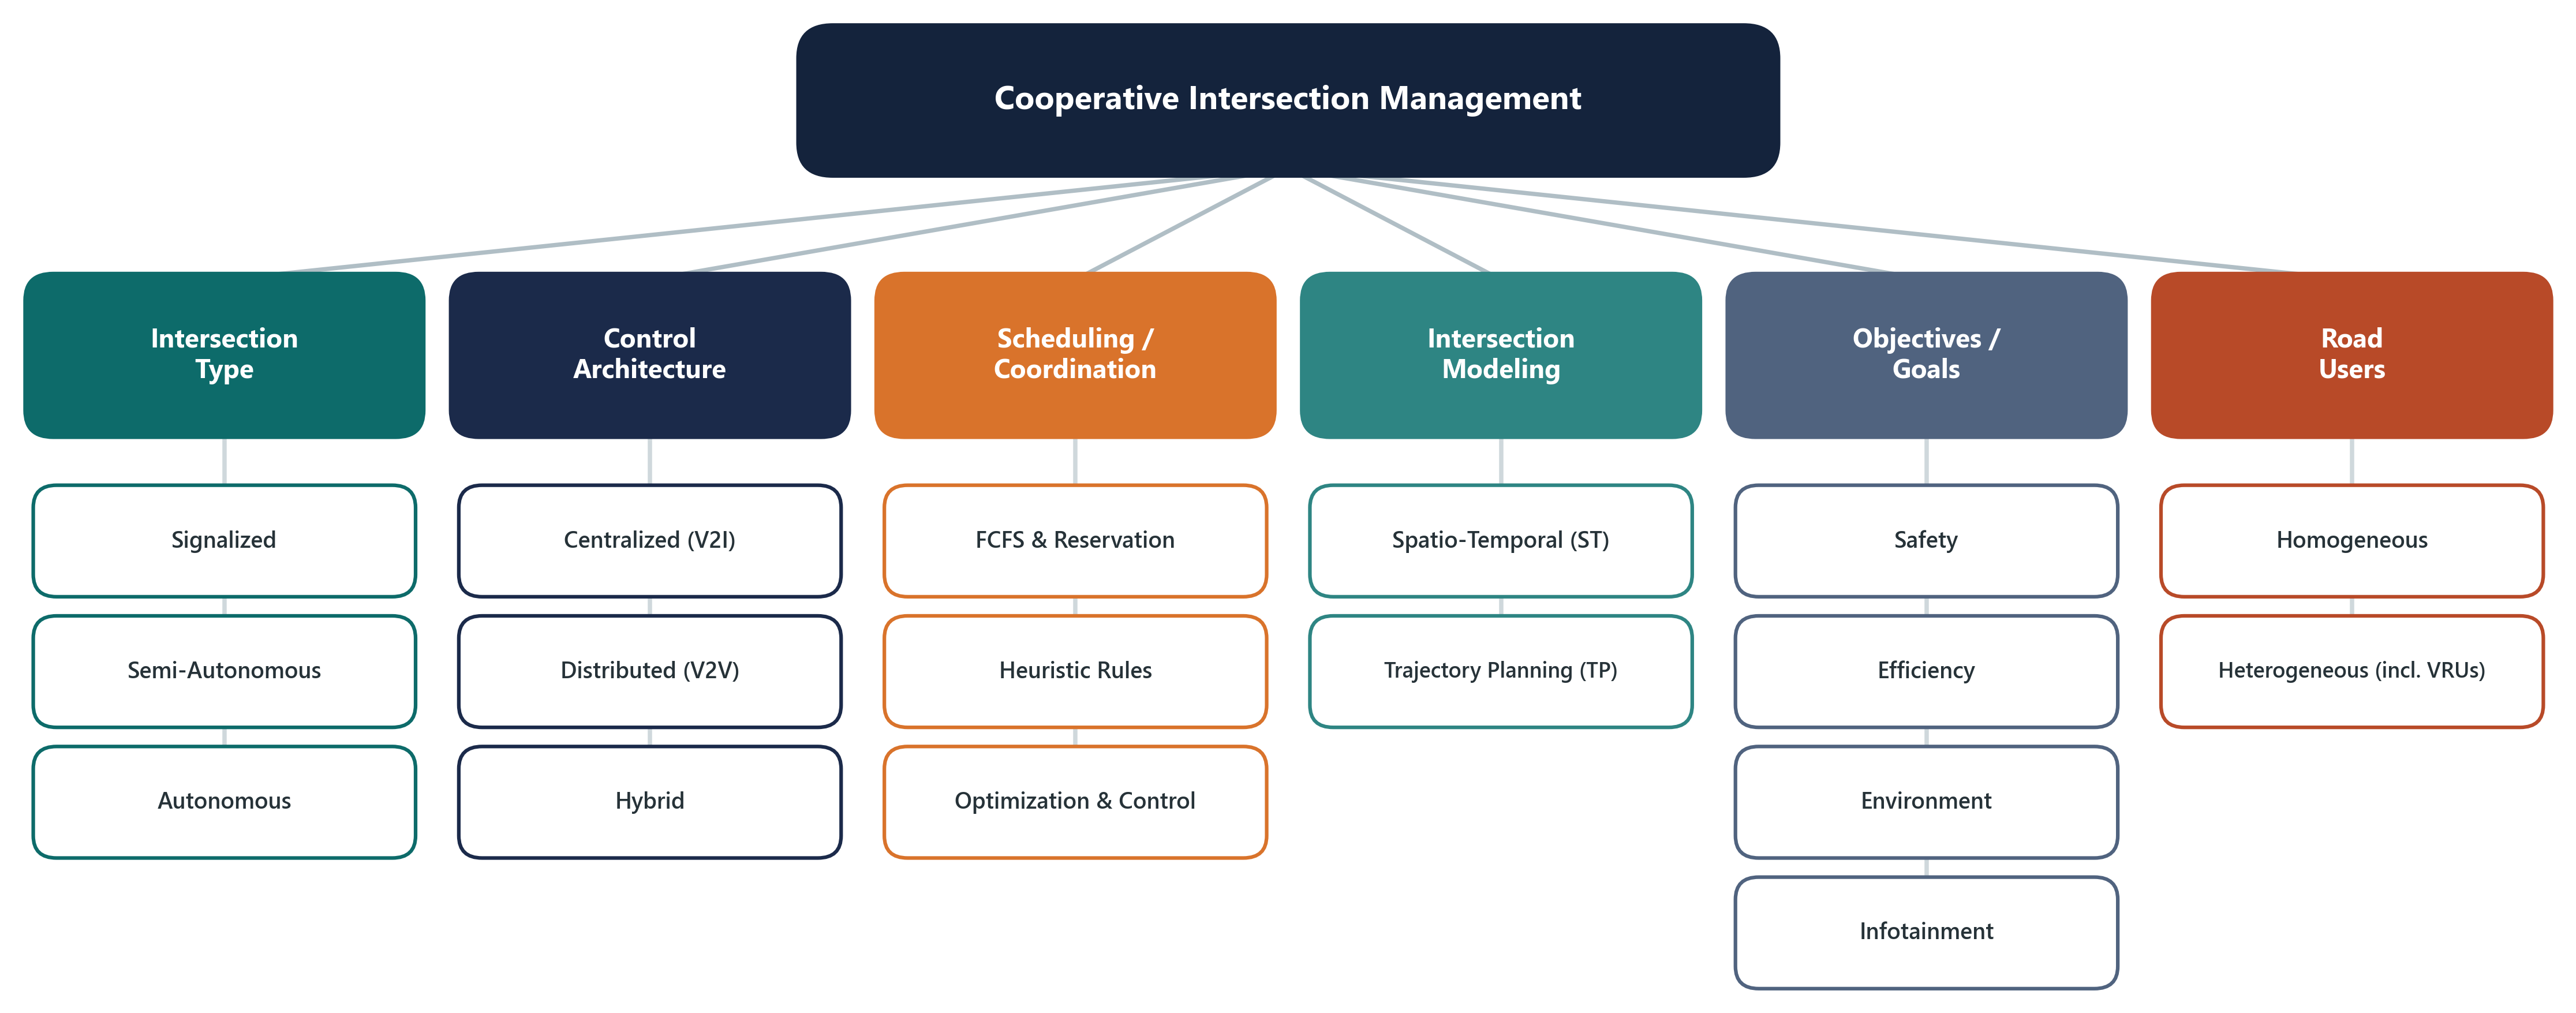
\includegraphics[width=\linewidth, height=2.8cm, keepaspectratio]{figures/fig_taxonomy.png}
        \caption{5-Axis AIM Taxonomy}
    \end{subfigure}
    \hfill
    \begin{subfigure}{0.44\textwidth}
        \centering
        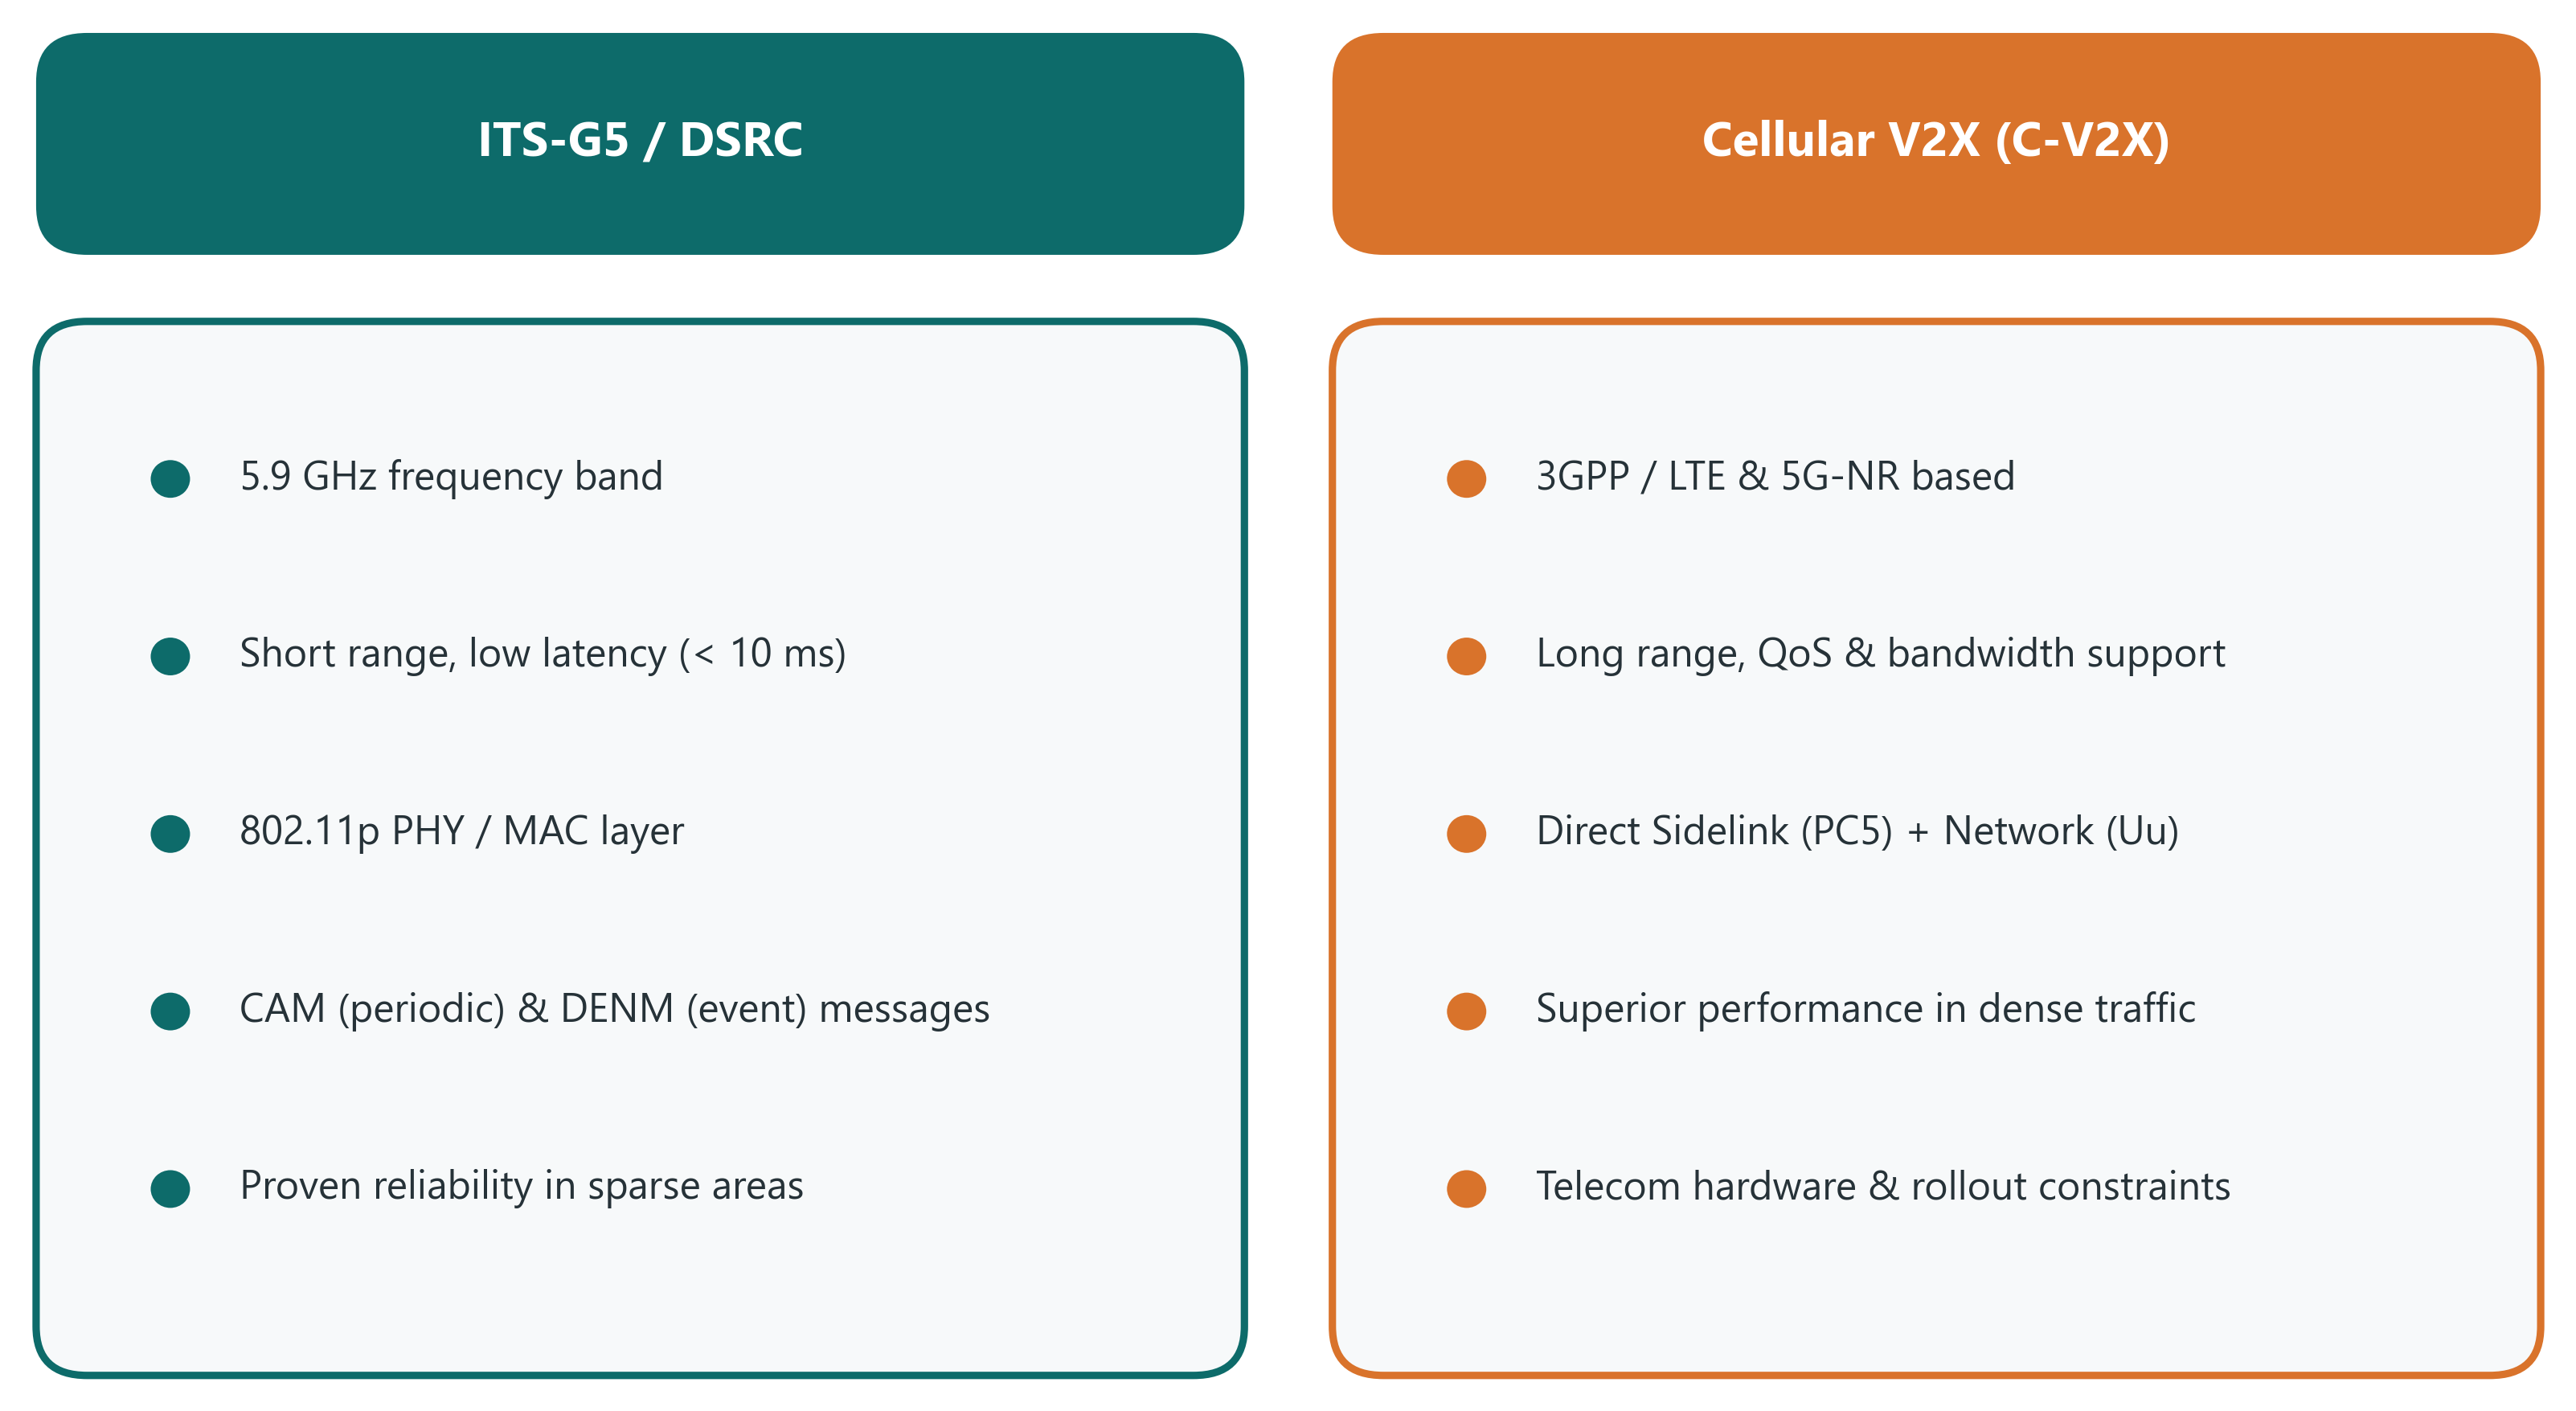
\includegraphics[width=\linewidth, height=2.8cm, keepaspectratio]{figures/fig_v2x.png}
        \caption{Connected Systems \& V2X Infrastructure}
    \end{subfigure}
    \vspace{-0.2cm}
    \caption{Hierarchical Taxonomy of Autonomous Intersection Management across Five Structural Dimensions.}
    \label{fig:master_taxonomy}
\end{figure}

\vspace{-0.2cm}
\section{DRL for Flow Stabilization: Insights from Ring Networks}
Foundational research in traffic reinforcement learning demonstrated that a single autonomous vehicle could dampen stop-and-go shockwaves in closed ring networks governed by the Intelligent Driver Model \cite{wu2017flow} (\autoref{fig:ring_dynamics}). By penalizing fleet velocity variance:
\begin{equation}
    r_{\text{ring}} = -\|v_{\text{fleet}} - v_{\text{target}}\|_2 - \lambda \cdot \text{Var}(v_{\text{fleet}})
\end{equation}
an RL agent acts as a moving bottleneck damper, decelerating proactively to absorb shockwaves and restoring uniform high-velocity equilibrium. This proved the capacity of DRL to regulate uncoordinated traffic.

\vspace{-0.2cm}
\begin{figure}[htbp]
    \centering
    \begin{subfigure}{0.48\textwidth}
        \centering
        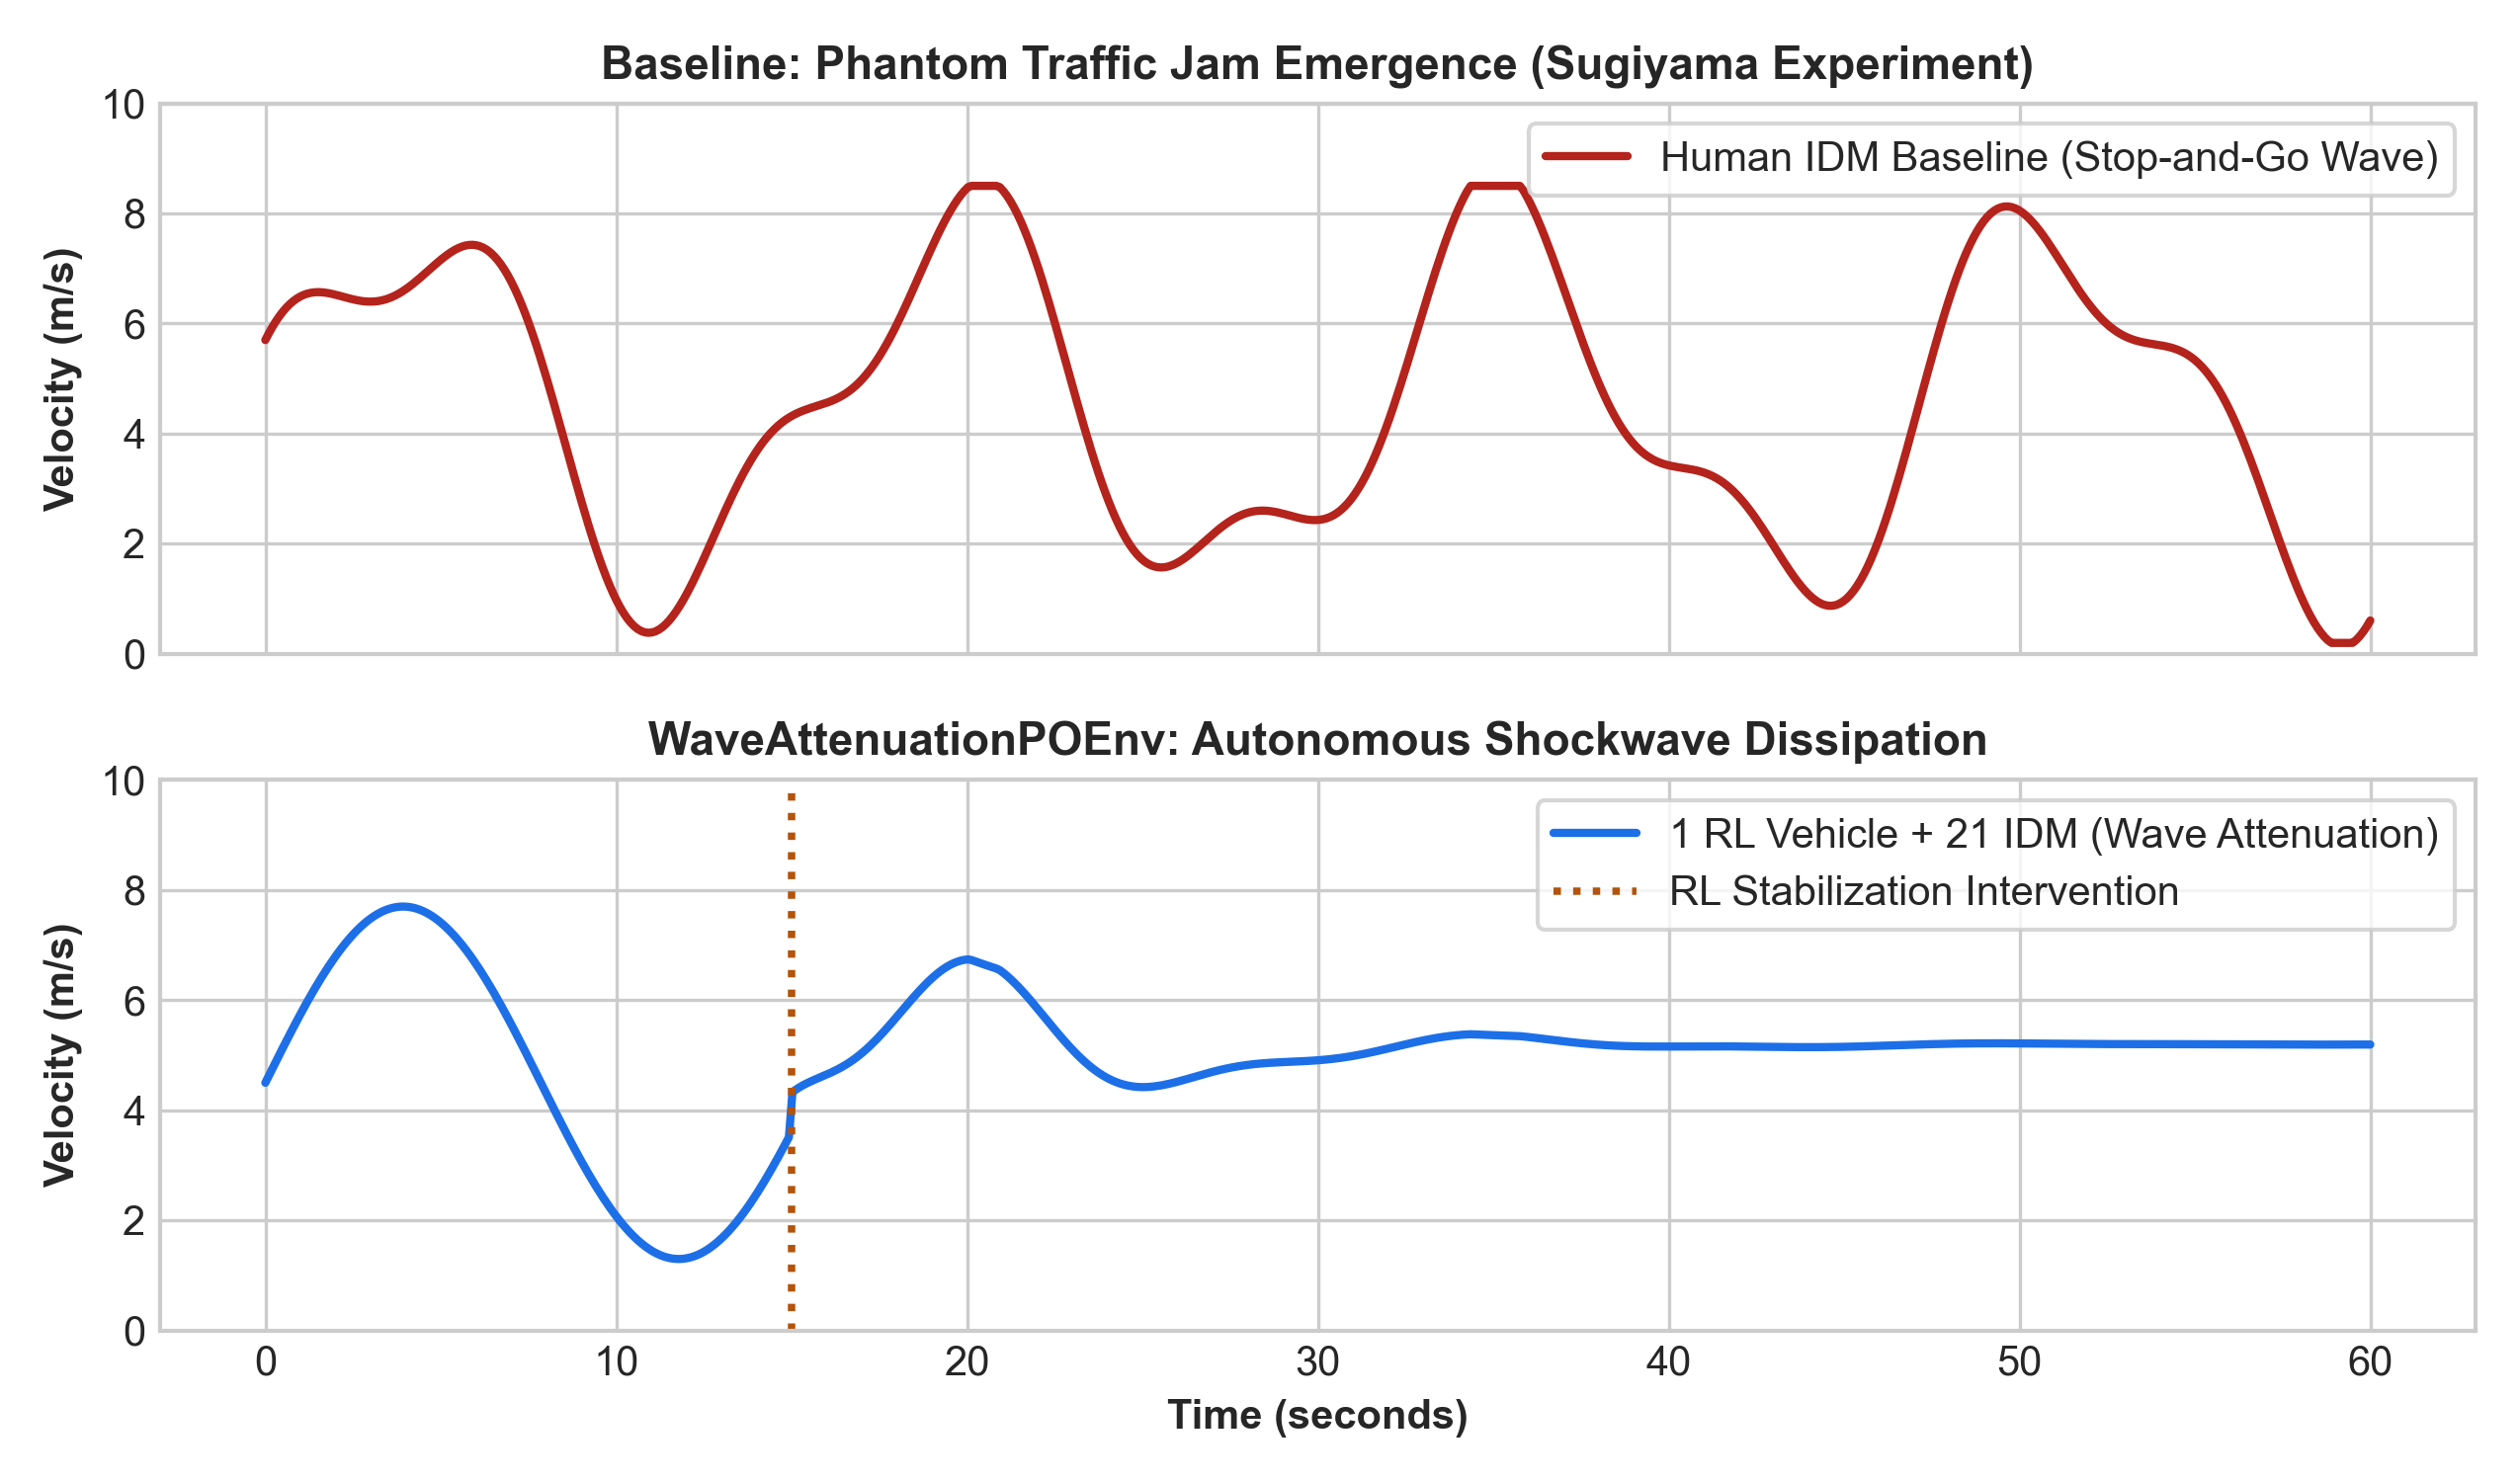
\includegraphics[width=\linewidth, height=2.7cm, keepaspectratio]{figures/ring_wave_attenuation_concept.png}
        \caption{Longitudinal Shockwave Damping}
    \end{subfigure}
    \hfill
    \begin{subfigure}{0.48\textwidth}
        \centering
        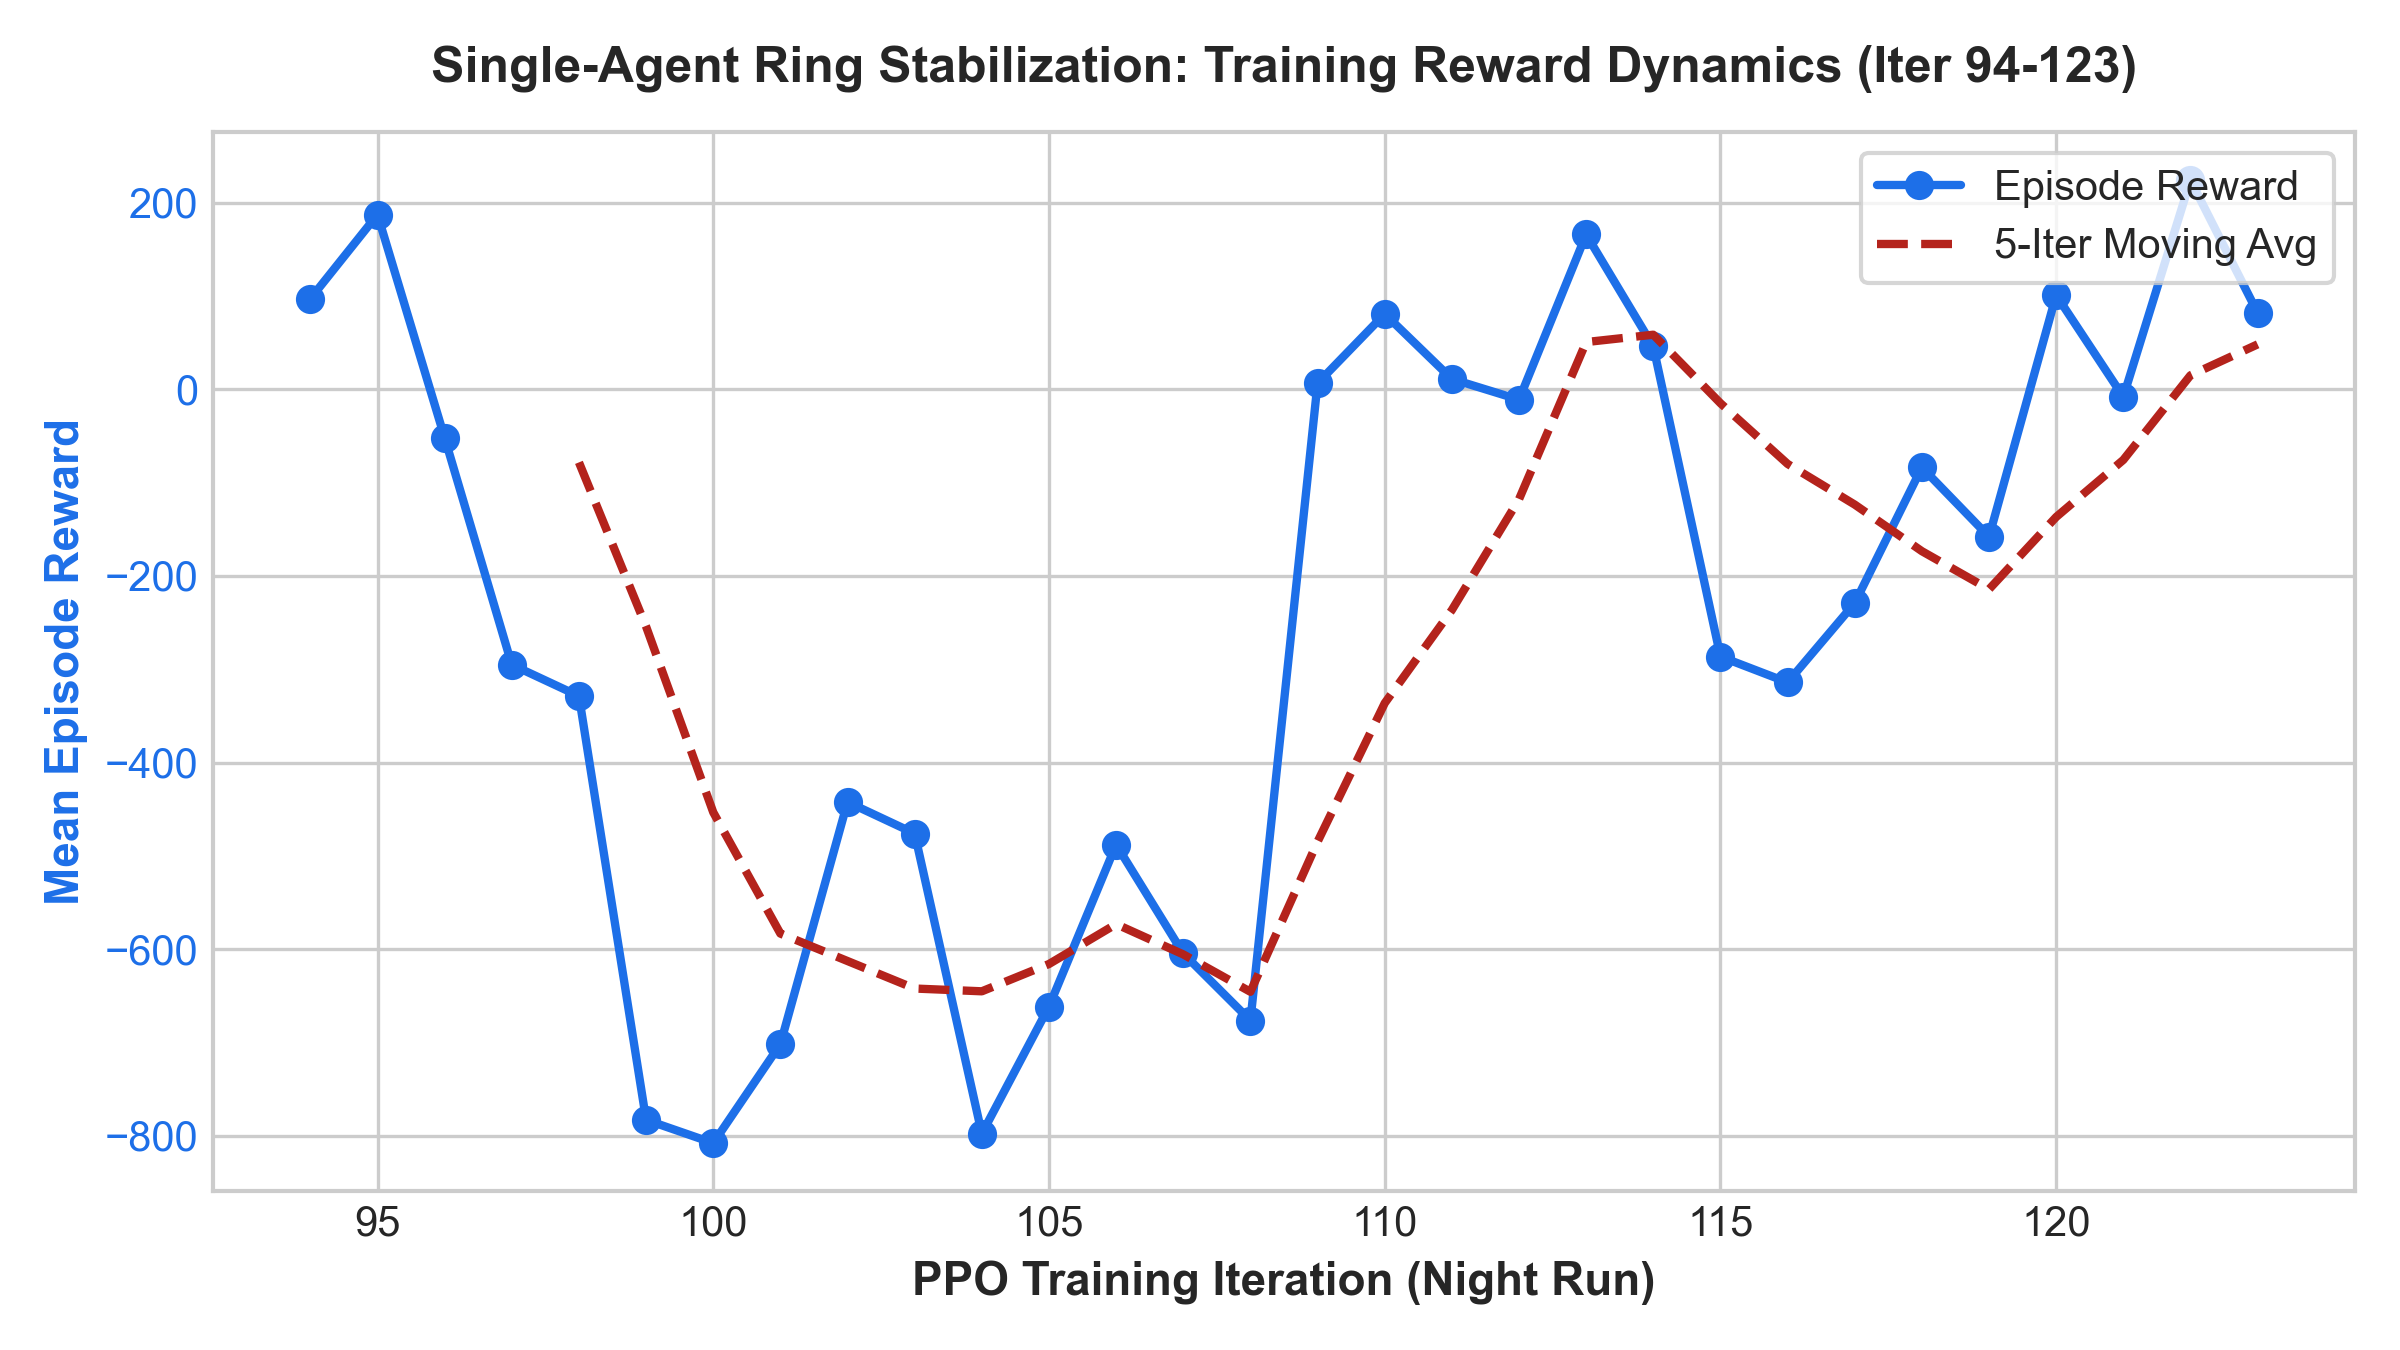
\includegraphics[width=\linewidth, height=2.7cm, keepaspectratio]{figures/ring_reward_dynamics.png}
        \caption{Reward \& Velocity Convergence}
    \end{subfigure}
    \vspace{-0.2cm}
    \caption{Shockwave Attenuation and DRL Velocity Regularization in Benchmark Ring Networks.}
    \label{fig:ring_dynamics}
\end{figure}

\vspace{-0.2cm}
\section{Unsignalized Intersection Navigation and the Multi-Task Dilemma}
In unsignalized intersections, the problem escalates to 2D collision avoidance across intersecting paths. While early studies restricted the agent to single maneuvers under occlusions \cite{isele2018navigating}, real-world deployment requires executing stochastic multi-task maneuvers (Left, Straight, Right). Xiao et al. \cite{xiao2024decision} addressed this dilemma by augmenting Soft Actor-Critic (SAC) with: (i) a task-intent feature $\mu_a$ encoding exit node orientation; (ii) a dual-dimension Mix-Attention network; and (iii) a segmented replay pool mitigating slow creeping policies. \autoref{tab:sota_matrix} provides a comparative synthesis benchmarking prior literature against our Phase 1 and Phase 2 implementations.

\begin{table}[htbp]
\centering
\footnotesize
\renewcommand{\arraystretch}{0.95}
\setlength{\tabcolsep}{3pt}
\resizebox{\textwidth}{!}{%
\begin{tabular}{|l|c|c|c|c|c|p{4cm}|}
\hline
\textbf{Study} & \textbf{Algorithm} & \textbf{Architecture} & \textbf{Multi-Task?} & \textbf{Simulator} & \textbf{Success Rate} & \textbf{Primary Limitation} \\ \hline
Dresner \& Stone \cite{dresner2008multiagent} & FCFS Heuristic & Centralized V2I & Yes & Custom & 100\% & Assumes 100\% CAV penetration and zero packet loss. \\ \hline
Isele et al. \cite{isele2018navigating} & Deep Q-Network & Autonomous Edge & Single (Left) & Kinematic & 93.4\% & Restricted to single maneuver under simplified traffic. \\ \hline
Zhong et al. \cite{zhong2021autonomous} & Survey / MPC & Centralized/Decent. & Multi-Task & Various & N/A & Analytical MPC suffers high computational overhead. \\ \hline
Gholamhosseinian \cite{gholamhosseinian2022comprehensive} & V2X Survey & Hybrid V2X & Multi-Task & Various & N/A & Highlights vulnerability to V2X communication latency. \\ \hline
Xiao et al. \cite{xiao2024decision} & Discrete SAC & Autonomous Edge & Yes (L/S/R) & \texttt{highway-env} & 97.4\% & 2D kinematic box environment without micro-yielding. \\ \hline
\textbf{This Work: Phase 1} & On-Policy PPO & Autonomous Edge & Yes (L/S/R) & Flow + SUMO & 94.9\% & On-policy sample inefficiency; left-turn timeouts. \\ \hline
\textbf{This Work: Phase 2} & Discrete SAC & Autonomous Edge & Yes (L/S/R) & Flow + SUMO & 99.52\% & Achieves 99.52\% crossing with 0.48\% collision rate. \\ \hline
\end{tabular}%
}
\vspace{-0.2cm}
\caption{Comparative Synthesis of Autonomous Intersection Management Literature and Project Phases}
\label{tab:sota_matrix}
\end{table}

\vspace{-0.2cm}
\section{Identified Research Gaps}
Our systematic survey identifies three core research gaps:
\begin{enumerate}
    \setlength{\itemsep}{0pt}\setlength{\parskip}{0pt}
    \item \textbf{The Kinematic-to-Microscopic Sim2Sim Gap}: Leading benchmarks (including Xiao et al. \cite{xiao2024decision}) evaluate in kinematic boxes (\texttt{highway-env}), overlooking microscopic car-following and right-of-way yielding dynamics in SUMO.
    \item \textbf{Specification Gaming in Sparse Rewards}: Discount factors ($\gamma < 1.0$) incentivize velocity maximization. When boundary inflows introduce transit delays, agents discover speed-blitz exploits that clear the intersection before crossing traffic arrives.
    \item \textbf{Multi-Core Architectural Stalls}: Microscopic simulations coupled with deep neural networks suffer acute OpenMP thread synchronization stalls on modern hybrid multi-core processors.
\end{enumerate}

